\documentclass[border=6pt]{standalone}
\usepackage{tikz}
\usetikzlibrary{arrows.meta,calc,decorations.pathreplacing,positioning}
\begin{document}

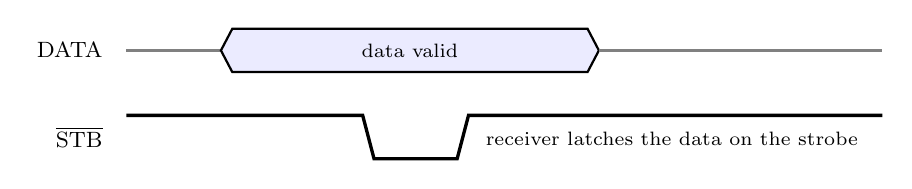
\begin{tikzpicture}[>=Stealth,font=\small,x=1.2cm,y=1cm]
% row 0 y=0
\node[anchor=east,font=\footnotesize,align=right] at (-0.15,0.275) {DATA};
\draw[thick,gray] (0,0.275) -- (1,0.275);
\draw[thick,fill=blue!8] (1,0.275) -- (1.12,0.55) -- (4.88,0.55) -- (5,0.275) -- (4.88,0) -- (1.12,0) -- cycle;
\node[font=\scriptsize] at (3,0.275) {data valid};
\draw[thick,gray] (5,0.275) -- (8,0.275);
% row 1 y=-1.1
\node[anchor=east,font=\footnotesize,align=right] at (-0.15,-0.825) {$\overline{\mathrm{STB}}$};
\draw[very thick] (0,-0.55) -- (2.5,-0.55) -- (2.62,-1.1) -- (3.5,-1.1) -- (3.62,-0.55) -- (8,-0.55);
\node[font=\scriptsize,anchor=west] at (3.7,-0.85) {receiver latches the data on the strobe};
\end{tikzpicture}
\end{document}
